\chapter{Basic machine learning schemes}
In our research, we use ensemble methods to predict future price change of limit order books. As comparisons, some basic machine learning tools,such as logistic regression, lasso and ridge regression and support vector machine,  are used. We call them "basic", not because they are simple, but because they have relatively long history and have already been widely used before. In the following, we give a brief introduction of these models.


\section{Logistic regression}
Logistic regression is a statistical tool which is used to find the fitting model to characterize the relationship between the independent variables and the response variable. Unlike traditional linear regression, the response variable of logistic regression is logit transformation of the probability. More clearly, suppose that we have a binary dependent variable $Y$, and we try to define the condition probability $Pr(Y=1|X=x)$, which denoted as $p(x)$. An unbounded range transformation, which is called \textbf{logistic} (or \textbf{logit}) \textbf{transformation} $log\frac{p}{1-p}$, is introduced. The advantage of \textbf{logit transformation} is that it is unbounded in both positive and negative direction when $p(x)$ approaches to 1 and 0 respectively. Formally, the formula of logistic regression model is as follows:\\
\begin{equation}\label{eq:logit}
log\frac{p(x)}{1-p(x)}=\beta_0+x\cdot \beta
\end{equation}      

Solving the above formula for $p$ will give us:


\begin{equation}\label{eq:logit_p}
p(x;b,\omega)=\frac{e^{\beta_0+x\cdot\beta}}{1+e^{\beta_0+x\cdot\beta}}=\frac{1}{1+e^{-(\beta_0+x\cdot\beta)}}
\end{equation}      
To solve the binary classification problem, we can assume $Y=1$ when $p>=0.5$ and $Y=0$ when $p<0.5$. Logistic regression is a widely used tool in applied statistics and discrete data analysis. There are some reasons for this:

\begin{itemize}
	\item It is a traditional and classical model with a relatively long history, which can be track back to \cite{bliss1934method}. It has a wide range of applications in a lot of areas, so there are many related materials and cases that one can refer to. 
	\item It has "exponential family" distribution property, which states that the probability of a specific variable $v$ can be described linearly by $exp\beta_0+\sum_{j=1}^{m}f_j(v)\beta_j$. If we let the vector $v$ as binary, 0 or 1, and the functions $f_j$ become all identical, then we can obtain a logistic regression. Exponential families take a very important role in statistical and physical research area, so it is beneficial if we turn a problem to logistic regression problem.  
	\item Contingency table plays a critical role in classification problem since if we take a contingency table with two columns(independent variable $Y$) and many rows(dependent variables $x$), the contingency table become the classification problem to some extent. Logistic regression gives a linear interpolation for the log-odds, so it is very helpful in the classification problem.  

\end{itemize}

Because the logistic regression deal with the probabilities, rather than just classes, we can use likelihood to fit the model.Assume that we have independent variable $Y$(denoted by $y_i$ for each data ) and dependent variables $x$(denoted by $x_i$ for each data), the probability is either $p$, if $y_i=1$, or $1-p$, if $y_i=0$. The Likelihood is defined as follows:
\begin{equation}\label{en:likelihood}
L(\beta_0,\beta)=\prod_{i=1}^{n}p(x_i)^{y_i}(1-p(x_i))^{1-y_i}
\end{equation}

Take $log$ transformation on both sides, the log-likelihood becomes:

\begin{equation}\label{en:log-likelihood}
\begin{aligned}
l(\beta_0,\beta)&=\sum_{i=1}^{n}y_i logp(x_i)+(1-y_i)log(1-p(x_i))\\
&=\sum_{i=1}^{n}log(1-p(x))+\sum_{i=1}^{n}y_ilog\frac{p(x)}{(1-p(x))}\\
&=\sum_{i=1}^{n}log(1-p(x_i))+\sum_{i=1}^{n}y_i(\beta_0+x\cdot \beta)\\
&=\sum_{i=1}^{n}-log(1+\exp^{\beta_0+x_i\cdot \beta})+ \sum_{i=1}^{n}y_i(\beta_0+x_i\cdot\beta)
\end{aligned}
\end{equation}

To find maximum of the log-likelihood, we can take first derivative of the log-likelihood function with respect to coefficient and set it equal to zero. The result is in the following:\\
\begin{equation}\label{en:likelihood_derivative}
\begin{aligned}
\frac{\partial l }{\partial \beta_j}&=-\sum_{i=1}^{n}\frac{1}{1+\exp^{(\beta_0+x_i\cdot \beta)}}\exp^{(\beta_0+x_i\beta)}x_{ij}
+\sum_{i=1}^{n}y_ix_{ij}\\
&=\sum_{i=1}^{n}(y_i-p(x_i;\beta_0,\beta))x_{ij}
\end{aligned}
\end{equation}

From equation \ref{en:likelihood_derivative}, we can see that it is a transcendental equation which can not transform to a polynomial equation, so there is no analytical solution. However we can solve it approximately with some numerical tools such as newton method and so on.   

\section{Lasso regression and ridge regression}
lasso and ridge regression add different regulation parameter to the ordinary least square regression, so before we describe lasso and ridge regression, we first give a short introduction of ordinary least square regression(OLS). Assume the response variable is $Y$ and the dependent variable is $x$, the following model: \\
\begin{equation}\label{en:ols}
y_i=\beta_0+x_{i1}\beta_1 +x_{i2}\beta_2+...+ x_{ik}\beta_k+e_i
\end{equation}
where $\beta_i$ corresponds to the coefficient of $x_i$ and $e_i$ is the error term with E[$e_i$]=0\\
is called least square regression. To make the error term become zero, we take the expectation on both sides and let $E(y_i)=\hat{y_i}$, now equation \ref{en:ols} becomes:
\begin{equation}
\begin{aligned}
E(y_i) &=\hat{y_i}=\beta_0+x_{i1}\beta_1 +x_{i2}\beta_2+...+ x_{ik}\beta_k\\
\hat{y} &={\bm{X\beta}}
\end{aligned}
\end{equation}

So the error term $\bm{e=Y-\hat{Y}}$ and we can define a loss function for the least square regression as $f=\bm{e'e}$. Our goal is to mimnimized this loss function. To realize this ,we can first define the loss function according to $\beta,x,$ and $y$.
\begin{equation}
\begin{aligned}
f&=\bm{e'e}=\sum_{i=1}^{n}e_i^2=\sum_{i=1}^{n}(y_i-\hat{y}_i)^2\\
&=(y_i-\hat{y}_i)'(y_i-\hat{y}_i)\\
&=\bm{(y-\bm{x\beta})'(y-\bm{x\beta})}\\
&=\bm{y'y-\beta'X'y-y'X\beta+\beta'X'X\beta}\\
&=\bm{y'y-2y'X\beta+\beta'X'X\beta}
\end{aligned}
\end{equation} 
Now let the first derivative of loss function to the coefficient $\beta$ equal to zero, i.e. $\frac{\partial f}{\partial \beta}=0$. Since $\bm{y'y}$ is constant with respect to $\beta$, so $\bm{\frac{\partial y'y}{\partial \beta}}$ is a null vector with the length equal to the number of data sample. The derivative of the second tern is:\\
\begin{equation}
\bm{\frac{\partial (-2y'X\beta)}{\partial \beta}=-2X'y}
\end{equation}
For the third term:

\begin{equation}
\bm{\frac{\partial \beta'X'X\beta}{\partial \beta}=-2X'X\beta}
\end{equation}

Now let the derivative of loss function equal to zero, we obtain that:
\begin{equation}
\begin{aligned}
\bm{\frac{\partial f}{\partial \beta}=2X'X\beta-2X'y}=0
\end{aligned}
\end{equation}

So we have:
\begin{equation}
\begin{aligned}
\bm{\frac{\partial f}{\partial \beta}=2X'X\beta-2X'y}&=0\\
\bm{X'X\beta} &=\bm{X'y}\\
\bm{X'X\beta} &=\bm{X'y}\\
\bm{\hat{\beta} }&=\bm{(X'X)^{-1}X'y}
\end{aligned}
\end{equation}

The $\hat{\beta}$ is our fitted coefficients which make the loss function smallest. In fact the expectation of $\hat{\beta}$ will equal to $\beta$, we give the proof as follows:
\begin{equation}
\begin{aligned}
\bm{E(\beta)}&=\bm{E[(X'X)^{-1}X'y]}\\
&=\bm{(X'X)^{-1}X'E(y)}\\
&=\bm{(X'X)^{-1}X'[X\beta]}\\
&=\bm{\beta}
\end{aligned}
\end{equation}
	
For the least square regression, if the rank ($\bm{X}$) is equal to number of independent variables, then the solution system only have one solution $\hat{\beta}$. But when the rank($\bm(x)$) is greater than the number of independent variables, the system will have infinitely many solutions, which make the solutions lack of credibility. Furthermore, even rank($\bm{X}$) equals to the number of independent variables, but when the sample size is close to the number of independent variables, least square regression can have a very poor prediction results. 

How to overcome these problems? One way is to add some constraints to the least squares model, that is:
\begin{equation}
\min_{\beta\in \mathbb{R}^p}||y-X\beta||_{2}^{2}\ subject\ to\ \beta\in C
\end{equation}
for some $C\in \mathbb{R}^p$, where $p$ is the number of independent variables. Lasso regression and ridge regression are two famous examples that choose $C$ to $l_1$ norm region and $l_2$ norm region. More clearly:\\
Ridge regression:
\begin{equation}\label{en:ridge}
\min_{\beta\in \mathbb{R}^p}||y-X\beta||_{2}^{2}\ subject\ to\ ||\beta||_2\leq t 
\end{equation}
Lasso regression:
\begin{equation}\label{en:lasso}
\min_{\beta\in \mathbb{R}^p}||y-X\beta||_{2}^{2}\ subject\ to\ ||\beta||_1\leq t 
\end{equation}
We can rewrite equation \ref{en:ridge} and \ref{en:lasso} with the KKT conditions and duality as:\\
Ridge regression:
\begin{equation}\label{en:ridge_dual}
\min_{\beta\in \mathbb{R}^p}||y-X\beta||_{2}^{2}\lambda||\beta||_2 
\end{equation}
Lasso regression:
\begin{equation}\label{en:lasso_dual}
\min_{\beta\in \mathbb{R}^p}||y-X\beta||_{2}^{2}+\lambda||\beta||_1 
\end{equation}

To our best knowledge, lasso regression was introduced by \cite{tibshirani1996regression} and \cite{chen2001atomic}. \cite{hoerl1970ridge} was the first one to propose ridge regression. From figure \ref{fig:lasso} and figure \ref{fig:ridge}, we can see that the constraint sets for both ridge and lasso are convex. The $l_1$ norm causes sparsity of the estimated coefficients, that is, there are $\beta_j=0$ for many j in the set ${1,...,p}$, when the tuning parameter become large.  However, this is not the case in ridge regression, which will always generate non-zero estimators, when the tuning parameter changes.  
 
 
 \begin{figure}[hbtp]
 	\begin{center}
 		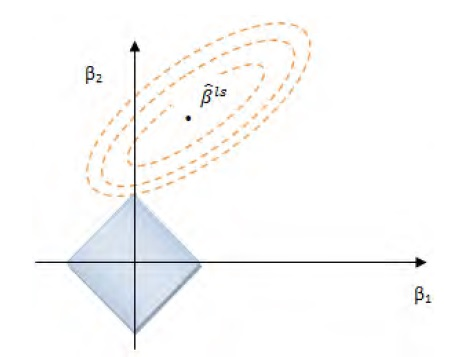
\includegraphics[width=3in,height=2.5in]{figures/lasso.jpg}
 	\end{center}
 	\caption{Illustration of Lasso constraints, redraw the chart in chapter 3 of \cite{friedman2001elements}} \label{fig:lasso}
 \end{figure}
 
 \begin{figure}[hbtp]
 	\begin{center}
 		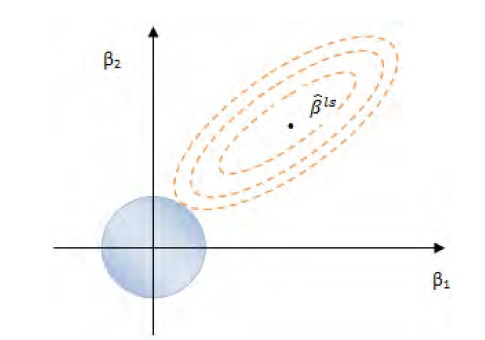
\includegraphics[width=3in,height=2.5in]{figures/ridge.jpg}
 	\end{center}
 	\caption{Illustration of Ridge constraints, redraw the chart in chapter 3 of \cite{friedman2001elements}} \label{fig:ridge}
 \end{figure}

From the KKT conditions(equation \ref{en:lasso_dual} and equation \ref{en:ridge_dual}), it is feasible to find the regression estimators as a function of $\lambda$, which is the tuning parameter. This is called \textit{solution path or regularization path} of the dual problem. Figure \ref{fig:lasso_path} and figure \ref{fig:ridge_path} show the regulation path of an example, we can see that lasso estimators will become zero when the tuning parameter rises. However, the ridge estimators will only approach to zero but never touch zero in most cases. 


\begin{figure}[hbtp]
	\begin{center}
		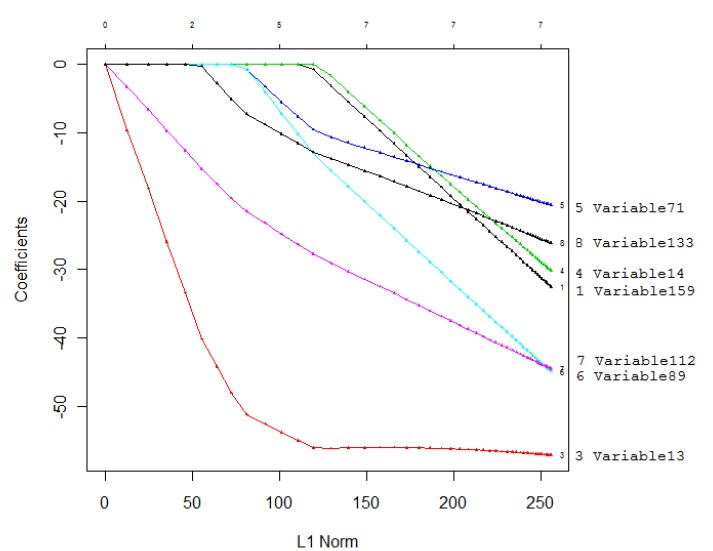
\includegraphics[width=3in,height=2.5in]{figures/lasso_p.jpg}
	\end{center}
	\caption{An example of the lasso regulation path with the increasing of the tuning parameter, each line represents the lasso solution , redraw the chart in chapter 3 of\cite{friedman2001elements}} \label{fig:lasso_path}
\end{figure}

\begin{figure}[hbtp]
	\begin{center}
		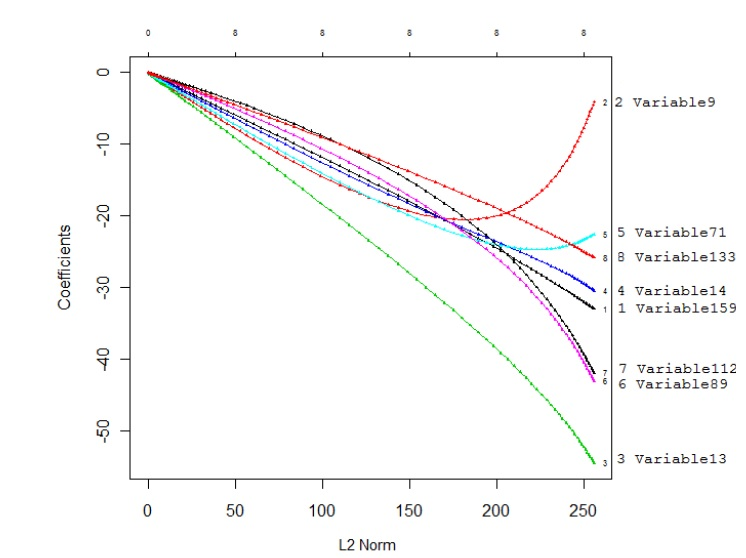
\includegraphics[width=3in,height=2.5in]{figures/ridge_p.jpg}
	\end{center}
	\caption{An example of the ridge regulation path with the increasing of the tuning parameter, each line represents the ridge solution , redraw the chart in chapter 3 of\cite{friedman2001elements}} \label{fig:ridge_path}
\end{figure}

\section{Support vector machine}
As far as we known, \cite{boser1992training} first introduced support vector machine(SVM) scheme, which is now widely used in bio-informatics, finance and other areas. Generally speaking, SVM is used to solve a linear two classes classification problem. Suppose there are input variables $x$ and output $y$ and we assume that $y$ only have two values: 1 for positive examples and -1 for negative examples. The relationship between $x$ and $y$ is:
\begin{equation}
f(x)=\sum_{i=1}^{N}\omega^T x +b
\end{equation} 
Where $\omega$ represents the \textit{weight vector}, and $b$ is known as the bias. The \textit{hyperplane} $\{x:f(x)=\omega^Tx+b\}$ divide the space into two side: when $f(x)=\omega^Tx+b>0$, we treat the data in the positive side and vice versa. The boundary that split the space into positive and negative is called the \textit{decision boundary}. Figure \ref{fig:svm_example} shows an example of decision boundary of SVM. The black line divide the data into two sets, the red data points are marked as positive and the blue ones are marked as negative. How to find the best decision boundary is the key problem in SVM learning process. To explain this, we need first introduce the definition of margin. When the decision boundary is defined, we denote the closet positive(negative) points to the hyperplane as $x_+(x_-)$. $\hat{\omega}$, the unit vector of $\omega$, is given by $\frac{\omega}{||\omega||}$ where $||\omega||$ is the norm of $\omega$. The margin of a decision boundary $f$ with respect to a dataset $\mathbb{D}$ can be defined as:
\begin{equation}
m_\mathbb{D}(f)=\frac{1}{2}\hat{\omega}^T(x_+-x_-)
\end{equation} 
Also we assume that the distance of $x_+$ and $x_-$ to the decision boundary $f$ is equal which means:
\begin{equation}\label{en:margin}
f(x_+)=\omega^Tx_++b=a\\
f(x_-)=\omega^Tx_-+b
\end{equation}
for some fixed number $a>0$ and $x_+$,$x_-$ can also called support vectors. To solve the margin, we set $a=1$ in euation \ref{en:margin}, add the two formula together and divide by $||\omega||$, we can get:
\begin{equation}
	m_\mathbb{D}(f)=\frac{1}{2}\hat{\omega}^T(x_+-x_-)=\frac{1}{||\omega||}
\end{equation}	


\begin{figure}[hbtp]
	\begin{center}
		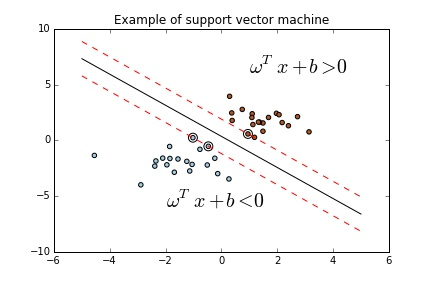
\includegraphics[width=4in,height=3.2in]{figures/svm_example.jpg}
	\end{center}
	\caption{Example of a linear support vector machine classifier. The black line is the decision boundary and the circled data are the support vectors.} \label{fig:svm_example}
\end{figure}
The goal of support vector machine scheme is to maximize the margin $\frac{1}{||w||}$, which is same as minimizing $||w||^2$. So the support vector machine problem can be transform to the following quadratic optimization problem:

\begin{equation}\label{eq:svm_optimization}
\begin{aligned}
& \underset{\omega,b}{\text{minimize}}
& &\frac{1}{2}||\omega||^2\\
& \text{subject to}
& & y_i(\omega^Tx_i+b)>=1, \; i = 1, \ldots, n.
\end{aligned}
\end{equation}

In the ideal case, the above equation can perfectly separate the data if they are linearly separable. However in practice, data is often not linearly separable, to allow errors we can replace the right side of equation \ref{eq:svm_optimization} with the following:
\begin{equation}
y_i(w^Tx_i+b)\geq1-\xi_i,\; i=1,\dots,n.
\end{equation}

where $\xi_i\geq0$ are called \textit{slack variables}. Under this condition, some misclassifications are allowed if the example lies in the margin and we call this kind of error a margin error. To penalize the margin errors and misclassification, equation \ref{en:svm_optimization} can be transformed to:
 
 \begin{equation}\label{eq:svm_optimization_margin}
 \begin{aligned}
 & \underset{\omega,b}{\text{minimize}}
 & &\frac{1}{2}||\omega||^2+C\sum_{i=1}^{n}\xi_i\\
 & \text{subject to}
 & & y_i(\omega^Tx_i+b)\geq 1-\xi_i, \; i = 1, \ldots, n,\xi_i\geq 0
 \end{aligned}
 \end{equation}
 
This formula is called \textit{soft margin} SVM, which was proposed by \cite{cortes1995support}. For solving this formula, we can use a lagrange multipliers method to obtain the dual form which utilize the inner product.

\begin{equation}
\begin{aligned}
& \underset{\alpha}{\text{maximize}}
& &\sum_{i=1}^{n}\alpha_i -\frac{1}{2}\sum_{i=1}^{n}\sum_{j=1}^{n}y_iy_j\alpha_i\alpha_jx_i^Tx_j\\
& \text{subject to}
& & \sum_{i=1}^{n}y_i\alpha_i=0,\; 0\leq\alpha_i\leq C
\end{aligned}
\end{equation}   
Here we use the formula $\omega=\sum_{i=1}^{n}y_i\alpha_ix_i$. 

As we mentioned before, in practice, the data is often non-linearly separable. To handle this problem, we often map our data from the input space $\mathcal{X}$ to a feature space $\mathcal{F}$. In the space $\mathcal{f}$, the data may be close to linear separable and the discriminant function in this space is:$f(x)=\omega^T\Phi(x)+b$. Suppose the weight vector can be represented by a linear combination of the training samples,i.e. $\omega=\sum_{i=1}^{n}\alpha_ix_i$
then:
\begin{equation}
f(x)=\sum_{i=1}^{n}\alpha_ix_i^Tx +b
\end{equation}

The above formula becomes the following form in the space $\mathcal{f}$

\begin{equation}\label{en:decision_phi}
f(x) =\sum_{i=1}^{n} \alpha_i\Phi(x_i)^T\Phi(x)+b
\end{equation} 
If we define a kernel function $k(x,x')$ as
\begin{equation}\label{kernel}
k(x,x')=\Phi(x)^T\Phi(x')
\end{equation}
then the equation \ref{en:decision_phi} can be written in terms of the kernel function:
\begin{equation}\label{decision_kernal}
f(x)=\sum_{i=1}^{n}\alpha_ik(x,x_i)+b
\end{equation}
The following is an example: let $\Phi(x)=(x_1^2,\sqrt{2}x_1x_2,x_2^2)^T$, if we use the kernel function: $k(x,x')=(x^Tx)^2$,then:
\begin{equation*}
\begin{aligned}
\Phi(x)^T\Phi(z)&=(x_1^2,\sqrt{2}x_1x_2,x_2^2)^T(z_1,\sqrt{2}z_1z_2,z_2^2)\\
&=x_1^2z_1^2+2x_1x_2z_1z_2+x_2^2z_2^2\\
&=(x^Tz)^2
\end{aligned}
\end{equation*}
We can see that the mapping function $\Phi$ maps the data $x$ in the low dimensional space to the data $\Phi(x)$ in the high dimensional space. The inner product of the high dimensional data is equal to the mapping results of the inner product of the low dimensional data under the kernel function.The following are some widely used types of kernel function.\\
Linear kernel: mapping function $\Phi$ is identity,i.e. no mapping
\begin{equation}
k(x,z)=x^Tz
\end{equation}
Polynomial kernel(with degree d):
\begin{equation}
k(x,z)=(x^Tz)^d\;or\;(1+x^Tz)^d
\end{equation}
Radial Basis function kernel:mapping the variable x to an infinite dimensional feature space.
\begin{equation}
k(x,z)=exp[-r||x-z||^2]
\end{equation}
There has 

\section{Decision tree}
Ensemble models combine some weaker classifiers to become a strong classifier. Decision tree is a commonly used weaker classifier. We also use decision tree result as the reference to our ensemble models. In the following, we give a brief introduction of decision tree learning scheme.
Decision tree learning is a method to approximate discrete target function. The learned function can be treated as decision processes which apply the if-then rules.
Decision trees classify examples by sorting them from the top root node to the bottom leaf node. Each node in the tree represents a test of one characteristic of the example and each branch from that node specifies one of the possible results for this characteristic
\begin{figure}[hbtp]
	\begin{center}
		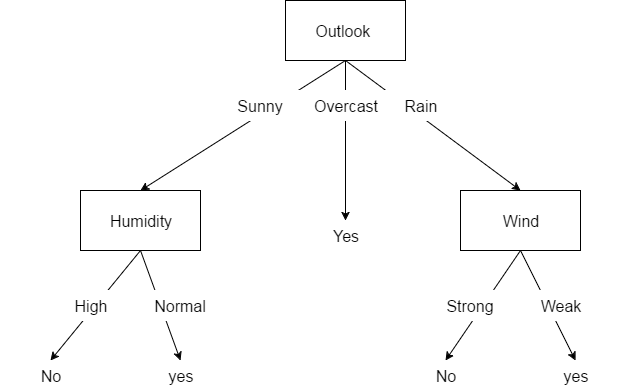
\includegraphics[width=5in,height=4in]{figures/dt_example.png}
	\end{center}
	\caption{Example of decision tree, determine if a person will go out for playing table tennis or not.Nodes are attributes of the weather in a given day and the output in the last layer is yes or not. } \label{fig:dt_example}
\end{figure}    

Figure \ref{fig:dt_example} gives us a illustration of a typical decision tree learning process. Given an instance (Outlook =Sunny,Temperature =Hot, Humidity=High and Wind =Weak), it will go down to he leftmost branch of this decision tree and will be classified negative,which will not go to tennis on this day.  

To improve the efficiency of the learning process, we would like to select the characteristic that is most helpful to classify the samples. We introduce a definition called "\textit{entropy}" which measures the degree of impurity in a given sample set. Suppose there is a data sample $S$, including positive and negative instances, the entropy of $S$ correspond to this binomial classification is :
\begin{equation}
Entropy(S)=-p_+log_2 p_+-p_-log2p_-
\end{equation} 

where the $p_+$ is the ratio of positive instances in sample $S$ and $p_-$ is the ratio of negative instances in $S$.For example, is a data set $S$ has 14 instances, in which 9 are positive and 5 are negative(we denote them as [$9+,5-$]). Then the entropy of $S$ is:
\begin{equation}\label{en:entropy}
\begin{aligned}
Entropy([9+,5-])&=-\frac{9}{14}log2 \frac{9}{14}-\frac{5}{14}log2 \frac{5}{14}\\
&=0.940
\end{aligned}
\end{equation}
More generally, if the target value takes more than 2 different classes,then the entropy of $S$ can be written as:
\begin{equation}	
Entropy(S) = \sum_{i=1}{C}-p_ilog2 p_i 	
\end{equation}

where $p_i$ represents the ratio of the number of samples with class i to the whole sample size and $C$ is the number of different classes. We now introduce another new definition that judge the effectiveness of a feature to classify the data sample and call it \textit{information gain}. More formally, information gain regard to a sample data $S$ is:
\begin{equation}
Gain(S,A)=Entropy (S) -\sum_{v\in Values(A)}^{\frac{|S_v|}{|S|}}Entropy(S_v)
\end{equation}

where $Values(A)$ is the collection of all possible values for feature $A$ and $S_v$ is the subset of $S$ where feature A has value $v$($S_v={s\in S|A(s)=v})$
Now let see an example of information gain. We still assume a collection $S$ including 14 instances [9+,5-] and the instances that have Wind=Weak contain 6 positive and 2 negative examples, the remainder have Wind = Strong. The information gain of sorting these 14 samples by the feature Wind can be obtained as :
\begin{equation}
\begin{aligned}
Values(Wind)&=Weak,Strong\\
S&=[9+,5-]\\
S_{Weak}&=[6+,2-]\\
S_{strong}&=[3+,3-]\\
Gain(S,Wind)&=Entropy(S)-\sum_{v\in Values(A)\in\{Weak,Strong\}}\frac{S_v}{S}Entropy(S_v)\\
&=Entropy(S)-(\frac{8}{14})Entropy(S_{Weak})-(\frac{6}{14})Entropy(S_strong)\\
&=0.940 -(\frac{8}{14})0.811-\frac{6}{14}1.00\\
&=0.048
\end{aligned}
\end{equation}
